\chapter{Mid fidelity prototype}

\section{Prototype}
The second prototype of the project is the Mid fidelity prototype. The improvement here is the interaction, the interface didn't change much other then some scaling and logo. We took some of the advice from the peer-review from the lo-fi prototype.\\
The prototype is made in balsamiq, a prototype mockup program.\\
Below is a screen-clipping of the welcome screen.
\begin{figure}[H]
\centering
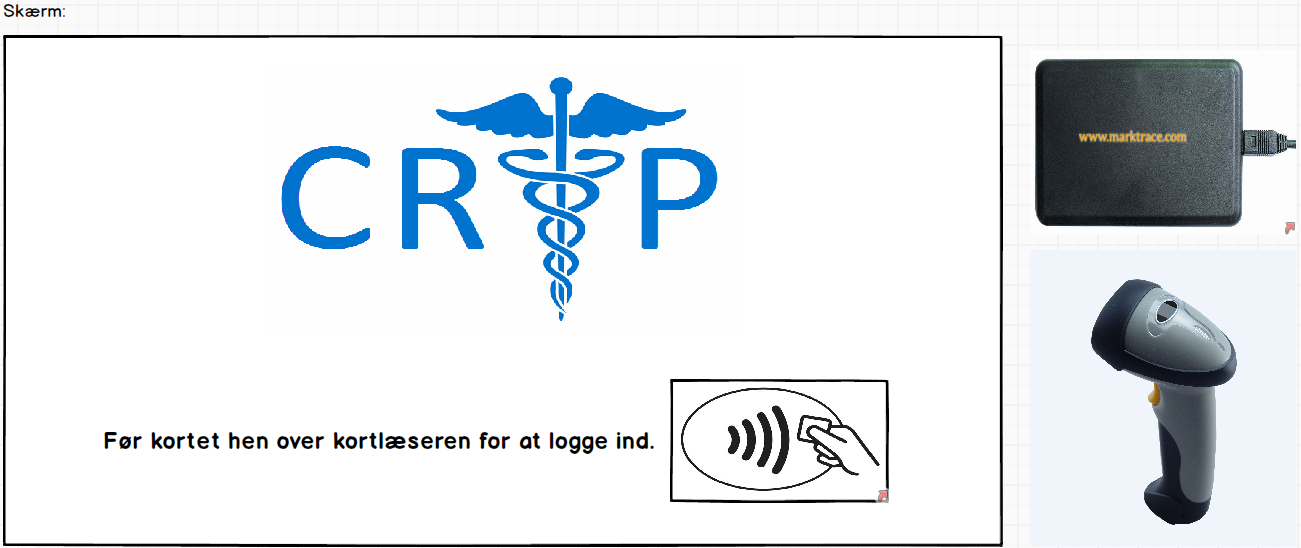
\includegraphics[width=.9\textwidth]{billeder/WelcomeScreen_MidFi}
\caption{Welcome screen in the mid-fi prototype}
\end{figure}
The pictures simulates the RFID scanner which makes it possible to login to the system. The prototype is made on a device with a touchscreen so it is possible to navigate the menus with touch.\\
In balsamiq you can link between different mockups so buttons can be used to navigate through the prototype.\\
So by tapping the RFID scanner the user logs into the system. Below is shown the first page upon login.\\
\begin{figure}[H]
\centering
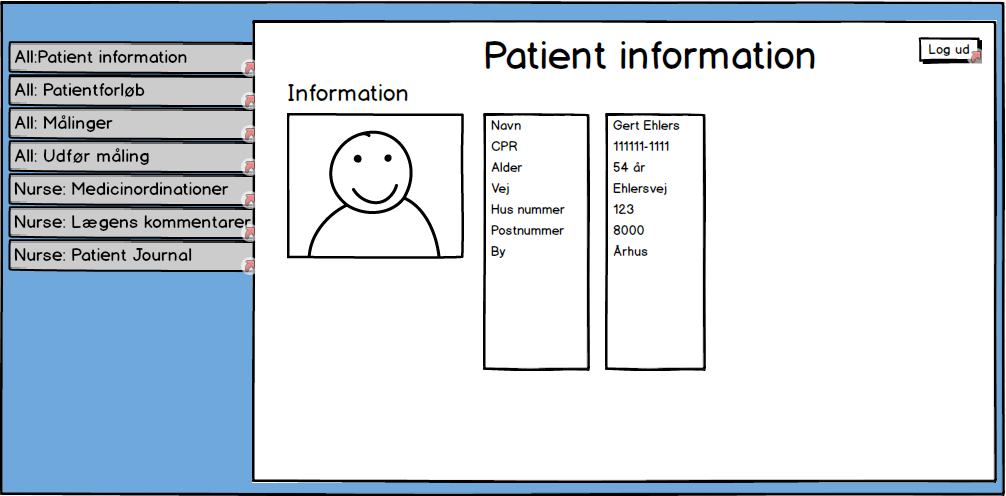
\includegraphics[width=.9\textwidth]{billeder/PatientInformation_MidFi}
\caption{First page, Patient Information, upon login to the CRIP system}
\end{figure}
The mid-fi prototype gives a better feel of the real product then the low-fi.\\
It does this because the navigation have a better feel and the prototype is visually pleasing.\\
The touch feature enables the user to use the prototype as intended which was not possible with the low-fi prototype.\\
In the peer reviews from the low-fi prototype we got some feedback which was applied to the mid-fi.\\

\section{Obtaining usability goals}
With the mid-fi prototype we aimed to give the user a more optimized version of our prototype in order to measure improvements. The buttons was made larger and more text was added so we could comply with our usability goals.

\section{Obtaining user experience goals}
The goal with the mid-fi prototype was to measure whether we had improved on our initial design. The time spent on navigating should be reduced as well as errors in navigation. The mid-fi is also closer to the final result we want and serves as a way of showing what we want to do.

\section{Peer review}
This peer review was performed in the same way as for the lo-fi peer review, and the same evaluation method was used. Different from the first review, only two persons did this review, and then we did a “speak aloud test” on a person with no knowledge of the system. With the data from the review, it is possible to see the learnability on the progress in time and navigation errors compared to the first review. The intention of the “speak aloud test” was to get design and usability comments from a new user, who tested the system for 5 minutes. \\
\subsection{Results of mid-fi peer review}
The peer review group who participated in the second review was even smaller than the first time, which affects the results to be less reliable. However, as the graph below show, the results have improved, and the system is easier for them to use. Besides the time on task, their comments was very useful again this time, and together with the “speak aloud test” we received new design ideas to improve in the hi-fi prototype. Among other ideas we will move the “log out” button to a more natural position and a suggestion to tiles at welcome screen was taken to consideration. \\

\begin{figure}[H]
\centering
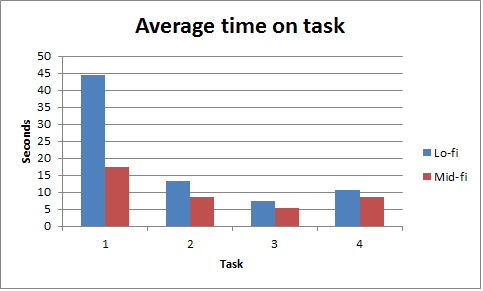
\includegraphics[width=.7\textwidth]{billeder/AverageTime}
\caption{Comparison of average time on tasks.}
\end{figure}
